% CVPR 2025 Paper Template; see https://github.com/cvpr-org/author-kit
% Place cvpr.sty and ieeenat_fullname.bst from the official author kit
% in this directory before compiling.

\documentclass[10pt,twocolumn,letterpaper]{article}

%%%%%%%%% PAPER TYPE  - PLEASE UPDATE FOR FINAL VERSION
% \usepackage{cvpr}              % To produce the CAMERA-READY version
\usepackage[review]{cvpr}      % To produce the REVIEW version
% \usepackage[pagenumbers]{cvpr} % To force page numbers, e.g. for an arXiv version

% Import additional packages in the preamble file, before hyperref
\usepackage{graphicx}
\usepackage{placeins}
\usepackage{float}
\usepackage{amsmath}
\usepackage{amssymb}
\usepackage{booktabs}
\usepackage{multirow}
\usepackage{xcolor}
\usepackage{colortbl}
\definecolor{oursrow}{RGB}{232,242,250}


% It is strongly recommended to use hyperref, especially for the review version.
% hyperref with option pagebackref eases the reviewers' job.
% Please disable hyperref *only* if you encounter grave issues, 
% e.g. with the file validation for the camera-ready version.
%
% If you comment hyperref and then uncomment it, you should delete *.aux before re-running LaTeX.
% (Or just hit 'q' on the first LaTeX run, let it finish, and you should be clear).
\definecolor{cvprblue}{rgb}{0.21,0.49,0.74}
\usepackage[pagebackref,breaklinks,colorlinks,allcolors=cvprblue]{hyperref}

%%%%%%%%% PAPER ID  - PLEASE UPDATE
\def\paperID{23415} % *** Enter the Paper ID here
\def\confName{CVPR}
\def\confYear{2027}

%%%%%%%%% TITLE - PLEASE UPDATE
\title{HMamba-eMOT: Hypergraph Modulated State Updating in Mamba for RGB-Event Multi-Object Tracking} 

%%%%%%%%% AUTHORS - PLEASE UPDATE
\author{First Author\\
Institution1\\
Institution1 address\\
{\tt\small firstauthor@i1.org}
% For a paper whose authors are all at the same institution,
% omit the following lines up until the closing ``}''.
% Additional authors and addresses can be added with ``\and'',
% just like the second author.
% To save space, use either the email address or home page, not both
\and
Second Author\\
Institution2\\
First line of institution2 address\\
{\tt\small secondauthor@i2.org}
}

\begin{document}
\maketitle

\begin{abstract}
Multi-Object Tracking (MOT) is essential for autonomous driving and intelligent surveillance. State-of-the-art RGB trackers struggle under challenging conditions such as blur and overexposure, while event cameras provide complementary high dynamic range, asynchronous visual cues. However, effective RGB-event fusion and relational target association remain open problems. This paper proposes HMamba-eMOT, a two-stage multimodal MOT framework. We first introduce bidirectional Hypernetwork Linear Attention (HyLA) to dynamically generate modality-aware weights for adaptive cross-modal fusion before the YOLOX detection head. We further build a frame-level hypergraph to model spatial and appearance correlations across targets. Inspired by \(M^3\)amba, we leverage the hypergraph prior to residually modulate the \(\Delta\) and C matrices inside bidirectional Mamba, rather than simply concatenating hypergraph context with motion inputs. A two-stage association module outputs the final tracking results. Evaluations on DSEC-MOT and FEMOT demonstrate the effectiveness of our approach.
%% 
\textcolor{red}{Source code will be released upon acceptance.} 
\end{abstract}





\section{Introduction}

Multi-Object Tracking (MOT), a fundamental task in computer vision and artificial intelligence that aims to localize multiple objects and maintain their identities over time, is widely demanded in autonomous driving, intelligent transportation, robotics, and video surveillance.  
Current trackers fall into two groups, i.e., \textit{query-based} and \textit{detector-based MOT methods}.  
The query-based methods carry identity in a learned query and update it across frames, like MOTR~\cite{zeng2022motr}, MOTRv2~\cite{zhang2023motrv2}, MeMOTR~\cite{gao2023memotr}, MOTIP~\cite{gao2025motip}, and FEMOTR~\cite{wang2026femot}. 
Detector-based methods first localize objects and then associate the resulting boxes, as in ByteTrack~\cite{zhang2022bytetrack}, FairMOT~\cite{zhang2021fairmot}, OC-SORT~\cite{cao2023ocsort}, and MambaTrack~\cite{huang2024mambatrack}. 
Both groups have advanced substantially on large-scale benchmarks~\cite{milan2016mot16,dendorfer2020mot20,sun2022dancetrack,yu2020bdd100k}. 
Equipped with strong object detectors, discriminative appearance embeddings, and effective target-association strategies, they now perform reliably in many well-conditioned scenes. 


Despite these advances, robust tracking under challenging conditions still remains a challenging problem. Low illumination, backlighting, occlusion, crowded scenarios, camera jitter, and fast-moving targets pose severe challenges to conventional fixed-rate RGB cameras, which capture texture and color information with a fixed shutter. Such adverse conditions readily induce motion blur and overexposure, corrupting the appearance cues that trackers rely on for object detection and re-identification, and eventually leading to accumulated association errors along trajectories.


Event cameras provide complementary visual measurements. Asynchronously capturing pixel-wise brightness changes with microsecond-level latency and a high dynamic range~\cite{gallego2022event}, they preserve object contours even under motion blur or saturation, whereas RGB cameras supply dense appearance information crucial for identity discrimination. This makes frame-event sensing a promising paradigm for MOT. Nevertheless, research on RGB-event MOT is still in its early stage, with numerous open challenges remaining to be addressed. First, effective fusion between synchronous RGB frames and asynchronous event streams remains a long-standing bottleneck. Second, it is still an open problem for multi-object tracking frameworks to exploit the correlations among the spatial locations and semantic features of different targets for accurate association. Accordingly, this motivates our core research question: how can we design an RGB-event multi-modal MOT framework to realize high-performance object detection and candidate matching? 


To mitigate the open challenges in RGB-Event MOT, we propose a two-stage tracker, termed HMamba-eMOT. For multi-modal detection, we employ bidirectional Hypernetwork Linear Attention (HyLA) to facilitate cross-modal communication between RGB frames and event streams prior to the YOLOX head~\cite{ge2021yolox}. HyLA dynamically generates modality-specific weights from multi-modal features, so each modality can adaptively exploit complementary information from the other, rather than simply combining features. For motion modeling, we build a frame-level hypergraph to capture spatial and appearance correlations among targets and propagate motion cues between related objects. Unlike HyperSSM, which applies hypergraph operations on SSM inputs, our design is inspired by $M^3amba$~\cite{jing2026m3amba}: we use hypergraph context as a relational prompt to residually modulate the $\Delta$ and $C$ branches of bidirectional Mamba without altering the raw motion sequence. This strategy differentiates our method from straightforward feature concatenation and embeds inter-object relational priors into Mamba’s state update. A two-stage association module then outputs the final tracking results. Extensive evaluations on DSEC-MOT and FEMOT confirm the efficacy of our framework. 




To sum up, the main contributions of this paper can be summarized as follows:
\begin{itemize}
\item For RGB-event multimodal fusion, we propose a hypernetwork linear attention (HYLA) module, which dynamically generates modality-adaptive weights conditioned on cross-modal features to refine RGB and event representations. 
\item For the subsequent association stage, we introduce a hypergraph structure to model spatial and semantic correlations among objects within the same frame. The learned hypergraph prior is leveraged to modulate the state matrices $\Delta$ and $C$ inside the Mamba SSM, yielding high-quality candidate matches and boosting overall MOT performance. 
\item Comprehensive evaluations on the DSEC-MOT and FEMOT benchmark datasets demonstrate the superiority of our proposed HMamba-eMOT.  
\end{itemize}




\section{Related Work}

\subsection{Multi-Object Tracking}

Existing MOT methods fall into three groups: tracking-by-detection, joint detection and tracking, and query-based transformers. Tracking-by-detection trains a detector on still images and then links boxes. The link is a bipartite match~\cite{jonker1987lap} whose cost may use motion~\cite{cao2023ocsort}, appearance~\cite{wojke2017deepsort}, or both. ByteTrack~\cite{zhang2022bytetrack} adds a second round over low-score boxes. Joint detection-and-tracking methods, such as FairMOT~\cite{zhang2021fairmot}, predict the box and an embedding in one network, so a separate re-identification model is unnecessary. Our association stays with the two-round IoU schedule.

Query-based transformers carry identity in a track query. MOTR~\cite{zeng2022motr}, MOTRv2~\cite{zhang2023motrv2}, and MeMOTR~\cite{gao2023memotr} update that query through a decoder, and FEMOTR~\cite{wang2026femot} uses the same decoder on RGB-event input. They rely less on a hand-designed matcher, at the cost of clip-wise training and a slow decoder at test time. State-space models are a lighter temporal predictor. Mamba~\cite{gu2023mamba} writes its hidden state through input-dependent scan parameters, and MambaTrack~\cite{huang2024mambatrack} runs a bidirectional Mamba on box differences inside a tracking-by-detection matcher. We continue from that predictor. The added piece is a frame-level hypergraph: its context does not replace the box history, and it modulates $\Delta$ and $C$.

\subsection{RGB-Event Fusion}

RGB-event fusion has been studied for detection and for single-object tracking. Tomy~\emph{et al.}~\cite{tomy2022fusion} convert the asynchronous event stream into a frame and fuse it with RGB features at several detector stages. VisEvent~\cite{wang2024visevent} uses the frame for appearance and the events for motion in single-object tracking. AFNet~\cite{zhang2023afnet} aligns a low-rate frame with high-rate events and fuses the two by cross-correlation. CEUTrack~\cite{tang2026ceutrack} feeds color frames and event voxels to one Transformer, so extraction, fusion, and matching share a backbone. Mamba-FETrack~\cite{huang2024mambafetrack} uses a Mamba backbone for each modality and a further Mamba block to mix them. These tasks localize one target. MOT also requires the fused features to stay stable enough for association under occlusion and inter-object interaction.

On the two benchmarks, FEMOTR~\cite{wang2026femot} is the RGB-event multi-object tracker: it treats the frame as a low-frequency appearance signal and the event frame as a high-frequency contour, and fuses the two by amplitude and phase attention before a query decoder. PFTrack~\cite{zhu2025pftrack} is the other dual-modal method in the comparison, and it progressively fuses a visible image with a thermal image. The remaining rows marked RGB-Event in Tables~\ref{tab:femot} and~\ref{tab:dsec} are RGB trackers evaluated with both inputs. GTR, SiamMOT, ByteTrack, Trackformer, and SpikeMOT appear on DSEC-MOT with events alone. Our fusion stays inside a tracking-by-detection detector: HyLA lets each modality read the other, and relations among tracks are handled later by the hypergraph on the motion model.

\subsection{Hypernetwork and Hypergraphs}

A hypernetwork generates the weights of another network from a context vector~\cite{ha2017hypernetworks}. Schug~\emph{et al.}~\cite{schug2025hyla} show that multi-head attention already has this form. The scores across heads are a low-dimensional latent code, and that code generates the value transformation. Their operator strengthens this view of attention. It normalizes the code across heads in place of a softmax over keys, and it applies the same code twice, with a ReLU between the two contractions, so the generated value map is nonlinear. We use this operator so that the RGB and event streams can read each other inside the detector. The event cue therefore enters the RGB descriptor before any track edge is built.


A hypergraph generalizes pairwise connectivity. An ordinary graph edge joins two vertices, so a message is only the other endpoint. A hyperedge joins an arbitrary subset. Zhou, Huang, and Sch\"olkopf~\cite{zhou2006hypergraph} build a hypergraph Laplacian from the incidence matrix and use it for clustering, embedding, and label propagation, which keeps each group as one subset. Neural models turn the same incidence into a layer. HGNN~\cite{feng2019hgnn} passes messages from vertices to hyperedges and back to vertices. Hypergraph attention~\cite{bai2021hypergraph} then assigns a weight to each member of an edge, while HyperGCN~\cite{yadati2019hypergcn} replaces a hyperedge by a small graph so that a graph convolution can be applied.

In one frame the useful group is often larger than a pair: every track inside a spatial radius, or every track in one appearance component. We build those two hyperedges and aggregate the other members of each edge by their mean, the unweighted form of the vertex-edge-vertex pass. HyperSSM~\cite{song2026hyperssm} also uses a hypergraph for multi-object tracking, and applies it to the state-space input and state. Our context leaves the box history unchanged and modulates $\Delta$ and $C$.




\section{Methodology}

\subsection{Overview}

As shown in Figure~\ref{fig:overview}, HMamba-eMOT has two stages. The detector takes a paired RGB frame and event stream. Each modality is encoded by its own CSPDarknet, ordered as a stem and DarkNet blocks 1--3; the ellipsis between block 1 and block 3 stands for block 2. Before the YOLOX neck, bidirectional HyLA fuses the two streams independently at the three blocks. A shared residual MLP maps both streams into one channel space, and Hypernetwork Linear Attention then exchanges them. The inset returns the enhanced maps $F'_{\mathrm{rgb}}$ and $F'_{\mathrm{e}}$, and their gated sum is the single feature that enters the PA-FPN and the YOLOX head. The appearance memory is pooled from $F'_{\mathrm{rgb}}$ at block 1, before this sum.

The tracker reads the motion sequence of each track. It builds spatial and appearance hyperedges on the current frame, and a hypergraph convolution aggregates each group into a context vector. This context modulates the discretization step size $\Delta$ and the output matrix $C$ of three bidirectional Mamba blocks, which predict the next box. The context is not appended to the scanned sequence, and the input matrix $B$ is left unmodulated. Two-stage IoU association~\cite{zhang2022bytetrack} then links the predicted boxes to the new detections and writes the output tracks.


\begin{figure*}[t]
  \centering
  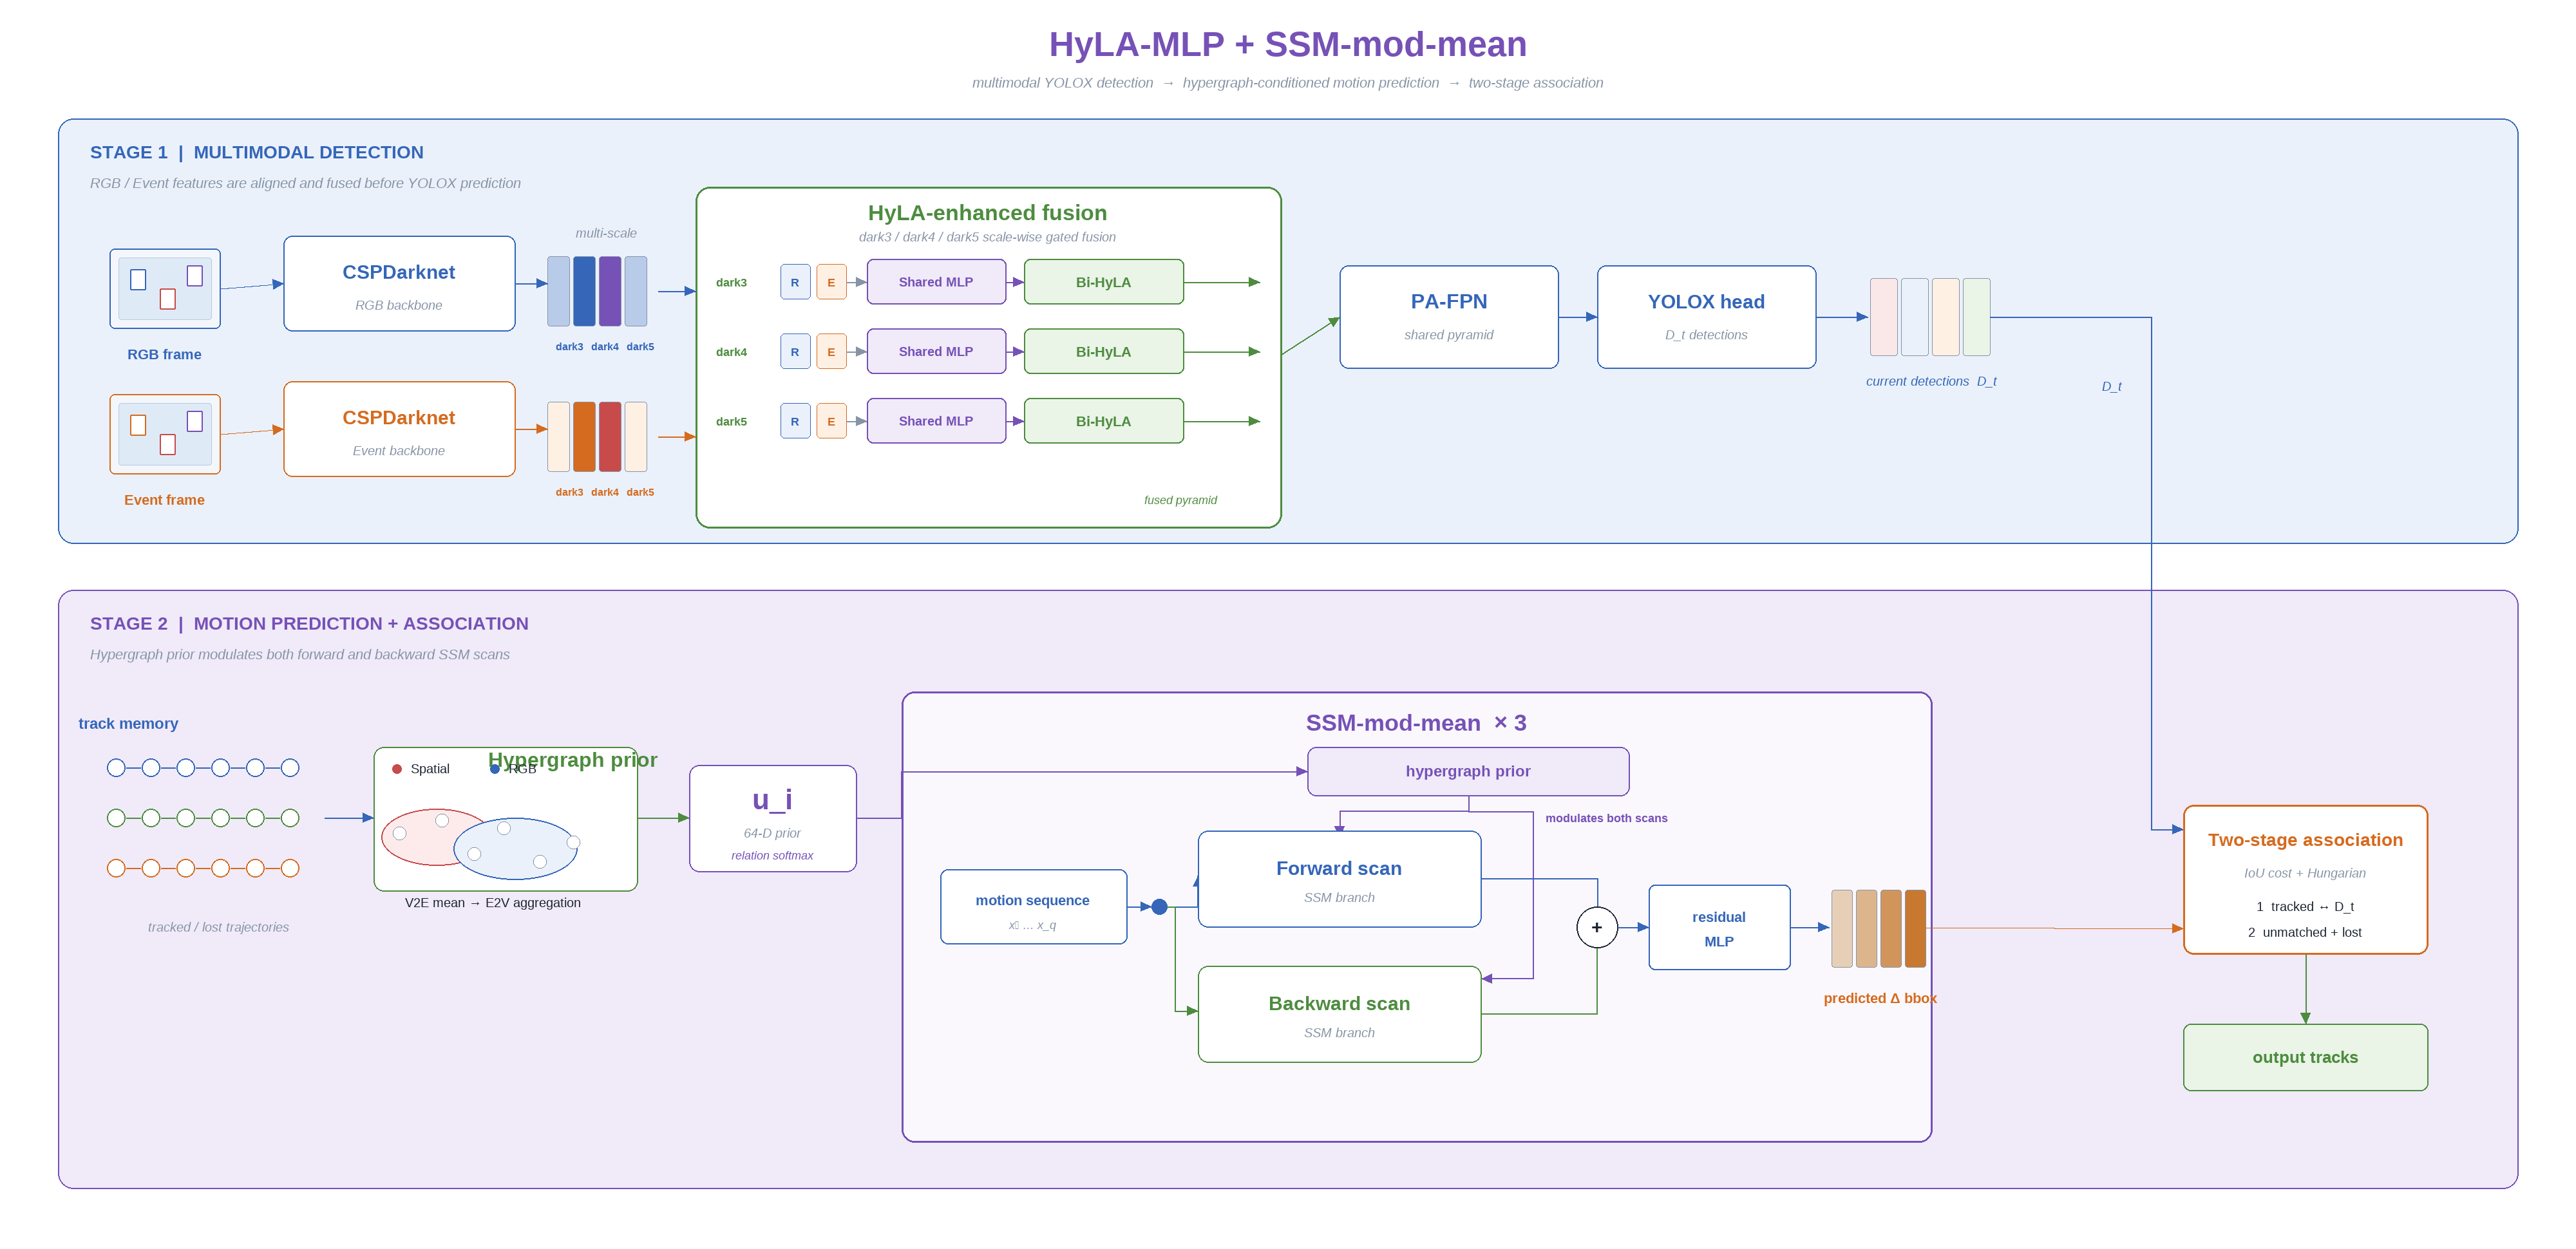
\includegraphics[width=\textwidth]{overall_framework.png}
  \caption{An overview of the proposed two-stage tracker HMamba-eMOT. In the detection stage, an RGB frame and an event stream pass through separate stems and DarkNet blocks 1--3. Bidirectional Hypernetwork Linear Attention fuses the two modalities at these blocks before the YOLOX neck. In the motion-inference stage, a hypergraph models the spatial and appearance relations among targets in the current frame, and this group prior modulates $\Delta$ and $C$ inside Mamba. Two-stage IoU association produces the final tracks.}
  \label{fig:overview}
\end{figure*}




\subsection{Network Architecture} 

\textbf{Shared-MLP HyLA detector.}
Each modality is encoded by its own CSPDarknet. Fusion is applied independently at blocks 1, 2, and 3, and the three fused maps enter one PA-FPN. At each block, the RGB and event backbone maps pass through one shared residual MLP,
\begin{equation}
\operatorname{MLP}(x)=x+W_2\,\mathrm{SiLU}\big(\mathrm{BN}(W_1 x)\big).
\end{equation}
$W_1$ and $W_2$ are $1\times1$ convolutions. $W_1$ expands the channel count by $2$. $W_2$ is zero-initialized, so the block starts as the identity. The same weights are applied to both modalities. Writing $R$ and $E$ for the backbone maps, the aligned maps are $F_{\mathrm{rgb}}=\mathrm{MLP}(R)$ and $F_{\mathrm{e}}=\mathrm{MLP}(E)$.

The joint query is the channel concatenation $J=[F_{\mathrm{rgb}};F_{\mathrm{e}}]$. For a context map $C\in\{F_{\mathrm{rgb}},F_{\mathrm{e}}\}$, GroupNorm with one group is applied to $J$ and to $C$, and $1\times1$ convolutions give
\begin{equation}
Q=W_q\,\mathrm{GN}(J),\qquad K=W_k\,\mathrm{GN}(C),\qquad V=W_v\,\mathrm{GN}(C).
\end{equation}
The maps are split into windows. Blocks 1 and 2 use $7\times7$ windows, and block 3 uses one global window. Inside a window the tokens are split into $4$ heads. The widths of $Q$, $K$, and $V$ are $64$, $96$, and $128$ at the three scales. The score of head $h$ between query token $q$ and key token $k$ is
\begin{equation}
S_{hqk}=\frac{Q_{hq}^{\top}K_{hk}}{\sqrt{d}},
\end{equation}
where $d$ is the head dimension. RMS normalization is taken over heads,
\begin{equation}
A_{hqk}=\frac{S_{hqk}}{\sqrt{\mathrm{mean}_{h}(S_{hqk}^{2})+\epsilon}},\qquad \epsilon=10^{-6}.
\end{equation}

The value network in Figure~\ref{fig:overview} applies these scores twice, with a ReLU between the two contractions~\cite{schug2025hyla}. The first contraction sums over heads,
\begin{equation}
U_{qkd}=\mathrm{ReLU}\Big(\sum_{h} A_{hqk}V_{hkd}\Big),\qquad
Y_{qhd}=\sum_{k} A_{hqk}U_{qkd}.
\end{equation}
In matrix form this is $U=\mathrm{ReLU}(AV)$ and $Y=AU$. Heads are concatenated and the windows are folded back. A $1\times1$ projection $W_o$ returns the channel width of the context map, and a zero-initialized scale adds the result back,
\begin{equation}
F'_{\mathrm{rgb}}=F_{\mathrm{rgb}}+a_{\mathrm{rgb}}W_o Y_{\mathrm{e}},\qquad
F'_{\mathrm{e}}=F_{\mathrm{e}}+a_{\mathrm{e}}W_o Y_{\mathrm{rgb}}.
\end{equation}
$Y_{\mathrm{e}}$ is computed with $C=F_{\mathrm{e}}$ and $Y_{\mathrm{rgb}}$ with $C=F_{\mathrm{rgb}}$. The scales $a_{\mathrm{rgb}}$ and $a_{\mathrm{e}}$ are initialized at zero.

The neck receives one fused map. Its inputs are $F'_{\mathrm{rgb}}$ and $F'_{\mathrm{e}}$, mixed by a sigmoid gate and a zero-initialized correction,
\begin{align}
g&=\sigma(W_g[F'_{\mathrm{rgb}};F'_{\mathrm{e}}]),\\
F &= F'_{\mathrm{rgb}} + F'_{\mathrm{e}} + W_F\big([g\odot F'_{\mathrm{rgb}};\,(1-g)\odot F'_{\mathrm{e}}]\big).
\end{align}
$W_F$ is zero-initialized. The tracker uses $F'_{\mathrm{rgb}}$ at block 1, before this gate, and the RGB hyperedge uses only that descriptor. The sum-fusion baseline replaces the block by an element-wise sum of the two backbone maps.


\textbf{Relational hypergraph.}
At every frame the predictor sees the tracked and lost trajectories, indexed by $i=1,\ldots,n$. Each trajectory contributes its latest box center $c_i$ and its RGB appearance memory $f_i$. The center is divided by the image width and height, so $c_i$ lies in the unit square. One incidence matrix is built for the current frame and reused across the $q$ history steps.

The spatial rule takes the normalized centers as input. Track $i$ proposes the hyperedge
\begin{equation}
e_i^{(s)}=\{j:\lVert c_i-c_j\rVert_2\le 0.10\}.
\end{equation}
The index $j$ runs over the $n$ tracks, and $\lVert\cdot\rVert_2$ is the Euclidean distance in the unit square. The proposer belongs to its own edge. The proposal is kept when $|e_i^{(s)}|\ge 2$, and each surviving proposal is a separate hyperedge.

RGB hyperedges take the appearance memories as input. We use the HyLA-enhanced dark3 descriptor $F'_{\mathrm{rgb}}$ as $f_i$. Event context enters this descriptor through the value network $Y_{\mathrm{e}}$ before the edge is built. With $\hat f_i=f_i/\max(\lVert f_i\rVert_2,10^{-8})$ and cosine similarity $S_{ij}=\hat f_i^{\top}\hat f_j$, let $k=\min(5,n-1)$ and let $\mathcal{N}_k(i)$ be the $k$ other tracks of largest similarity to $i$. The RGB hyperedge uses the undirected adjacency
\begin{equation}
A_{ij}
=
\mathbf{1}[S_{ij}\ge 0.841]
\,\mathbf{1}[j\in\mathcal{N}_k(i)]
\,\mathbf{1}[i\in\mathcal{N}_k(j)],
\quad i\neq j.
\end{equation}
$\mathbf{1}[\cdot]$ equals $1$ when its argument is true and $0$ otherwise, so $A_{ij}=1$ only when the cosine is at least $0.841$ and the two tracks are mutual top-$k$ neighbors. Each connected component with at least two vertices is one hyperedge.



For a relation whose kept hyperedges are $e=1,\ldots,E$, the incidence matrix is
\begin{equation}
H_{ie}=\mathbf{1}[i\in e].
\end{equation}
$H_{ie}$ is $1$ when track $i$ belongs to hyperedge $e$. Spatial and RGB matrices take one column per kept hyperedge, in enumeration order, and unused columns are zero. 




The messages read vertex features $z_i\in\mathbb{R}^{64}$, obtained by mapping the latest box difference of track $i$ through a linear layer, LayerNorm and SiLU. For an edge $e$, the leave-one-out peer of vertex $i$ is
\begin{equation}
p_{ie}=\frac{d_e\mu_e-H_{ie}z_i}{\max(d_e-H_{ie},1)},
\quad
\mu_e=\frac{\sum_j H_{je}z_j}{\max(d_e,1)}.
\end{equation}
$d_e=\sum_j H_{je}$ is the number of tracks in edge $e$, and $\mu_e$ is their mean feature. Subtracting $H_{ie}z_i$ removes track $i$ itself, so $p_{ie}$ is the mean of the other members. Peers are passed through an MLP and averaged over the edges that contain $i$ and at least one other vertex. A second MLP yields one message per relation. Writing $c_i^{(s)}$ and $c_i^{(r)}$ for the spatial and RGB messages, a softmax gate mixes the relations that are present,
\begin{equation}
a_i=\mathrm{softmax}\big(\mathrm{MLP}([z_i;c_i^{(s)};c_i^{(r)}])\big),
\end{equation}
\begin{equation}
u_i=\gamma\,W_u\!\left(a_{is}c_i^{(s)}+a_{ir}c_i^{(r)}\right).
\end{equation}
The input of the gate is the concatenation of $z_i$ with the two messages. $a_i=(a_{is},a_{ir})$ holds the two gate weights, $W_u$ is a linear map, and $\gamma$ is a learnable scalar initialized at $0.1$. $u_i$ is the context passed to Mamba. Mean aggregation has no edge attention. Dropping a relation zeros its incidence, so that relation contributes no peers. 



\textbf{History-modulated Mamba.}
The box-difference history is embedded by a linear map from $4$ to $512$ and processed by three bidirectional Mamba blocks~\cite{gu2023mamba} with state size $16$. Each block sums a forward scan and a scan of the time-reversed input, then adds a residual MLP. The hypergraph vector $u_i$ is not added to this embedding. Let $x_{it}$ be the post-convolution token of track $i$ at history step $t$. Mamba forms the pre-activation step size $\widetilde\Delta_{it}$ and the matrices $B_{it}$ and $C_{it}$ by linear projections of $x_{it}$. The modulation input concatenates that token with the broadcast context,
\begin{equation}
f_{it}=[x_{it};u_i],
\end{equation}
and the adopted residuals are
\begin{align}
\widetilde\Delta'_{it}&=\widetilde\Delta_{it}+\alpha_{\Delta}\,\mathrm{MLP}_{\Delta}(f_{it}),\\
C'_{it}&=C_{it}\odot\big(1+\alpha_{C}\tanh(\mathrm{MLP}_{C}(f_{it}))\big).
\end{align}
$\alpha_{\Delta}$ and $\alpha_{C}$ are learnable scalars, and $\mathrm{MLP}_{\Delta}$ and $\mathrm{MLP}_{C}$ are small networks on $f_{it}$. The same prior can also scale the input matrix,
\begin{equation}
B'_{it}=B_{it}\odot\big(1+\alpha_{B}\tanh(\mathrm{MLP}_{B}(f_{it}))\big),
\end{equation}
where $\alpha_{B}$ and $\mathrm{MLP}_{B}$ are the corresponding scalar and network. The adopted model freezes $\alpha_B=0$, so $B$ is left unchanged. $\Delta$ keeps the additive residual above. The product used for $C$ is not applied to $\Delta$. Both rejections are measured in Table~\ref{tab:design}. The $\Delta$ branch has no tanh. The scan applies $\mathrm{softplus}(\widetilde\Delta'+b_{\Delta})$ internally. Each $\alpha$ is initialized at $0.1$, and the last linear layer of each MLP is initialized at zero, so modulation starts as the identity. A mask can restrict modulation to the last $k$ steps; $k=0$ means the residual is applied on the whole history. The reported model uses $k=0$, so $\Delta$ and $C$ modulate every step.

The head pools each sequence to $128$ channels, then maps $128\rightarrow64\rightarrow4$ with a LeakyReLU. The four outputs are a denormalized box offset added to the latest box. The temporal window is $q=10$.

\textbf{Online association.}
Detections below a score $\tau_f$ are discarded. A detection starts a new track only when its score is at least $\tau_n$. Round one associates the tracked set with cost threshold $\tau_1$ on $1-\mathrm{IoU}$. Round two associates unmatched tracked boxes plus lost boxes with threshold $\tau_2$. A lost track is deleted after $T_{\mathrm{lost}}$ unmatched frames. The motion offset replaces the last box only when the memory already holds at least $T_{\mathrm{en}}$ boxes. The reported operating point is $\tau_f=0.25$, $\tau_1=0.75$, $\tau_2=0.80$, $T_{\mathrm{lost}}=20$, $T_{\mathrm{en}}=2$, and $\tau_n=0.55$. The cost thresholds correspond to minimum IoUs of $0.25$ and $0.20$. The supplementary material records the search.

\subsection{Loss Function}

The detector and the motion model are trained separately, and association is not part of either loss. On anchors assigned by the YOLOX objective~\cite{ge2021yolox},
\begin{equation}
\mathcal{L}_{\mathrm{det}}=\lambda_{\mathrm{iou}}\,\mathcal{L}_{\mathrm{iou}}+\mathcal{L}_{\mathrm{obj}}+\mathcal{L}_{\mathrm{cls}}+\mathcal{L}_{\mathrm{L1}},
\end{equation}
with $\lambda_{\mathrm{iou}}=5$ and $\mathcal{L}_{\mathrm{iou}}=1-\mathrm{IoU}^{2}$. The motion loss is Smooth-L1 on the next-box offset,
\begin{equation}
\mathcal{L}_{\mathrm{mot}}=\mathrm{SmoothL1}(\hat\delta,\delta^{\ast}).
\end{equation}
The hypergraph and the $\Delta$ and $C$ residuals receive gradient through this offset. A batch whose Smooth-L1 exceeds $1.0$ is skipped. The supplementary material gives the anchor assignment and the schedule of $\mathcal{L}_{\mathrm{L1}}$.

\section{Experiments}



\begin{table*}
  \centering
  \small
  \setlength{\tabcolsep}{3.2pt}
  \caption{RGB-event tracking on FEMOT, ordered by publication date. Results other than MambaTrack, PlugTrack, UniTrack, PS-MOT, HyperSSM, and Ours are from Wang \emph{et al.}~\cite{wang2026femot}. \textbf{Bold} is best and \underline{underline} is second best.}
  \label{tab:femot}
  \begin{tabular}{clllcccccc}
    \toprule
    No. & Tracker & Modality & Source & HOTA$\uparrow$ & DetA$\uparrow$ & AssA$\uparrow$ & MOTA$\uparrow$ & MOTP$\uparrow$ & IDF1$\uparrow$ \\
    \midrule
    01 & TraDes~\cite{wu2021trades} & RGB-Event & CVPR 2021 & 12.6 & 9.4 & 17.3 & 7.8 & 73.7 & 11.0 \\
    02 & FairMOT~\cite{zhang2021fairmot} & RGB-Event & IJCV 2021 & 22.1 & 15.2 & 32.4 & 17.0 & \textbf{78.7} & 23.7 \\
    03 & ByteTrack~\cite{zhang2022bytetrack} & RGB-Event & ECCV 2022 & 36.3 & 35.4 & 38.1 & 38.0 & 73.7 & 44.3 \\
    04 & MOTRv2~\cite{zhang2023motrv2} & RGB-Event & CVPR 2023 & 29.5 & 22.6 & 39.6 & 20.3 & 75.4 & 33.3 \\
    05 & OC-SORT~\cite{cao2023ocsort} & RGB-Event & CVPR 2023 & 23.1 & 15.0 & 36.3 & 15.9 & \underline{77.8} & 25.0 \\
    06 & MixSort-Oc~\cite{cui2023sportsmot} & RGB-Event & ICCV 2023 & 32.4 & 29.4 & 36.4 & 33.7 & 76.3 & 39.8 \\
    07 & MixSort-Byte~\cite{cui2023sportsmot} & RGB-Event & ICCV 2023 & 32.1 & 36.9 & 28.6 & 36.0 & 72.9 & 37.1 \\
    08 & MeMOTR~\cite{gao2023memotr} & RGB-Event & ICCV 2023 & 44.0 & 40.2 & 49.0 & 45.4 & 76.9 & 54.9 \\
    09 & Hybrid-SORT~\cite{yang2024hybridsort} & RGB-Event & AAAI 2024 & 22.1 & 13.8 & 36.2 & 14.2 & 76.6 & 23.1 \\
    10 & SRTrack~\cite{li2024srtrack} & RGB-Event & AAAI 2024 & 38.5 & 35.8 & 42.0 & 40.8 & 76.0 & 47.0 \\
    11 & TLDMOT~\cite{chen2024tldmot} & RGB-Event & CVPR 2024 & 28.2 & 33.6 & 24.7 & 23.6 & 73.0 & 33.4 \\
    12 & MambaTrack~\cite{huang2024mambatrack} & RGB-Event & ACM MM 2024 & 40.6 & 47.2 & 35.7 & 47.2 & 75.3 & 48.1 \\
    13 & TOPICTrack~\cite{cao2025topictrack} & RGB-Event & TIP 2025 & 17.9 & 16.2 & 20.3 & 14.4 & 76.2 & 17.3 \\
    14 & Samba~\cite{segu2025samba} & RGB-Event & ICLR 2025 & 38.1 & 30.0 & \underline{49.1} & 33.7 & 75.8 & 48.1 \\
    15 & PFTrack~\cite{zhu2025pftrack} & RGB-Event & PR 2025 & 29.7 & 33.5 & 27.0 & 33.6 & 75.7 & 34.0 \\
    16 & MOTIP~\cite{gao2025motip} & RGB-Event & CVPR 2025 & 33.2 & 36.6 & 30.9 & 16.9 & 74.4 & 36.6 \\
    17 & PlugTrack~\cite{kim2026plugtrack} & RGB-Event & AAAI 2026 & 42.5 & 47.3 & 39.0 & 47.6 & 75.3 & 51.5 \\
    18 & UniTrack~\cite{galoa2026unitrack} & RGB-Event & ICLR 2026 & 37.9 & \underline{47.6} & 31.1 & 45.7 & 75.2 & 43.6 \\
    19 & HyperSSM~\cite{song2026hyperssm} & RGB-Event & CVPR 2026 & 40.5 & 42.5 & 39.3 & 47.6 & 76.3 & 49.0 \\
    20 & FEMOTR~\cite{wang2026femot} & RGB-Event & arXiv 2026 & \textbf{48.9} & 45.2 & \textbf{53.8} & \textbf{52.0} & 76.7 & \textbf{62.0} \\
    21 & PS-MOT~\cite{luo2026psmot} & RGB-Event & ECCV 2026 & 36.9 & 47.3 & 29.6 & 44.9 & 74.6 & 41.7 \\
    \rowcolor{oursrow}
    22 & HMamba-eMOT & RGB-Event & Ours & \underline{45.5} & \textbf{48.3} & 43.9 & \underline{51.3} & 75.6 & \underline{55.9} \\
    \bottomrule
  \end{tabular}
\end{table*} 

\subsection{Datasets and Evaluation Metric}

We evaluate on FEMOT~\cite{wang2026femot}, an RGB-event multi-object tracking set recorded with a DVS346 camera. It contains $100$ sequences, about $200$K frames, $14.58$K trajectories and $0.42$M boxes of people and vehicles, with paired RGB frames and events accumulated between exposure boundaries. We follow the released split of $70$ training, $10$ validation and $20$ test sequences. The motion model sees $32{,}341$ training frames and $5{,}011$ validation frames. The test set evaluated below has $76{,}192$ ground-truth boxes and $2{,}620$ identities. 


We also evaluate on DSEC-MOT, which provides object-track annotations on the paired frame-event recordings of the DSEC driving dataset~\cite{gehrig2021dsec}. The annotated objects cover seven categories: pedestrian, rider, car, bus, truck, bicycle and motorcycle.

Tracking is measured by TrackEval on each test set with HOTA~\cite{luiten2021hota}, its detection and association factors DetA and AssA, CLEAR MOTA and MOTP~\cite{bernardin2008clear}, IDF1~\cite{ristani2016idf1}, and the identity-switch count IDSW. Categories are collapsed into one class in our evaluations on both datasets, following the primary FEMOT protocol. Higher is better except for IDSW.

\subsection{Implementation Details}

The detector is YOLOX-X, initialized from COCO and trained at batch size $24$ in FP16 on $416\times416$ inputs. The motion model is adapted with Adam at $5\times10^{-5}$ and batch size $64$, using block-1 RoI descriptors taken after HyLA and before the gated sum. DSEC detectors predict seven categories and follow the same recipe, with sum fusion for the MambaTrack baseline and HyLA fusion for our method. All experiments use NVIDIA A800-80GB GPUs. The supplementary material gives the initialization, augmentation, and learning-rate schedules. 



\begin{table*}[t]
  \centering
  \small
  \setlength{\tabcolsep}{3pt}
  \caption{Tracking on DSEC-MOT. Rows 01-05 keep the order of Wang \emph{et al.}~\cite{wang2026femot}. The remaining rows are ordered by publication date. \textbf{Bold} marks the best value, including ties.}
  \label{tab:dsec}
  \begin{tabular}{clllccccc}
    \toprule
    No. & Tracker & Modality & Source & HOTA$\uparrow$ & DetA$\uparrow$ & AssA$\uparrow$ & MOTA$\uparrow$ & IDF1$\uparrow$ \\
    \midrule
    01 & GTR~\cite{zhou2022gtr} & Event & CVPR 2022 & 41.9 & 43.8 & 40.4 & 47.5 & 49.0 \\
    02 & SiamMOT~\cite{shuai2021siammot} & Event & CVPR 2021 & 49.1 & 47.4 & 51.4 & 44.4 & 59.1 \\
    03 & ByteTrack~\cite{zhang2022bytetrack} & Event & ECCV 2022 & 44.9 & 42.3 & 47.9 & 48.1 & 54.5 \\
    04 & Trackformer~\cite{meinhardt2022trackformer} & Event & CVPR 2022 & 45.9 & 47.2 & 45.0 & 48.6 & 56.2 \\
    05 & SpikeMOT~\cite{wang2025spikemot} & Event & IEEE Access 2025 & 52.5 & 49.5 & 55.7 & 54.7 & 62.9 \\
    \midrule
    06 & OC-SORT~\cite{cao2023ocsort} & RGB-Event & CVPR 2023 & 27.7 & 17.7 & 43.9 & 10.6 & 29.8 \\
    07 & MeMOTR~\cite{gao2023memotr} & RGB-Event & ICCV 2023 & 48.4 & 36.2 & 64.9 & 35.8 & 54.9 \\
    08 & MambaTrack~\cite{huang2024mambatrack} & RGB-Event & ACM MM 2024 & 59.2 & 53.8 & 65.5 & 57.5 & 71.5 \\
    09 & Samba~\cite{segu2025samba} & RGB-Event & ICLR 2025 & 55.4 & 46.4 & 66.5 & 50.3 & 64.9 \\
    10 & MOTIP~\cite{gao2025motip} & RGB-Event & CVPR 2025 & 37.2 & 32.2 & 43.3 & 17.8 & 42.8 \\
    11 & PlugTrack~\cite{kim2026plugtrack} & RGB-Event & AAAI 2026 & 59.5 & 53.9 & 66.1 & 57.8 & 71.8 \\
    12 & UniTrack~\cite{galoa2026unitrack} & RGB-Event & ICLR 2026 & 59.3 & 54.0 & 65.5 & 57.9 & 71.1 \\
    13 & HyperSSM~\cite{song2026hyperssm} & RGB-Event & CVPR 2026 & 49.9 & 39.6 & 63.2 & 35.5 & 57.1 \\
    14 & FEMOTR~\cite{wang2026femot} & RGB-Event & arXiv 2026 & 52.4 & 40.6 & \textbf{67.8} & 37.5 & 59.0 \\
    \rowcolor{oursrow}
    15 & HMamba-eMOT & RGB-Event & Ours & \textbf{60.7} & \textbf{54.5} & \textbf{67.8} & \textbf{60.2} & \textbf{73.9} \\
    \bottomrule
  \end{tabular}
\end{table*} 

\subsection{Comparison on Public Benchmarks}

\paragraph{Results on FEMOT.}
Table~\ref{tab:femot} compares our tracker with the RGB-event results of Wang \emph{et al.}~\cite{wang2026femot}. Ours reaches HOTA $45.5$, second to FEMOTR ($48.9$), and the highest DetA ($48.3$). Relative to our dual-modal MambaTrack baseline, HOTA improves by $4.9$, AssA rises from $35.7$ to $43.9$, IDF1 from $48.1$ to $55.9$, and MOTA from $47.2$ to $51.3$, while IDSW falls from $4{,}129$ to $3{,}220$. The gain is mainly association. Identities are still linked by IoU on predicted boxes, so the result stays below query-based methods that keep a temporal memory. The detector has $169.0$M parameters, and the full pipeline runs at $3.71$ frames per second on this split, against $2.07$ for the FEMOTR end-to-end pass.

\begin{table}
  \centering
  \small
  \setlength{\tabcolsep}{6pt}
  \caption{Wall-clock time on the FEMOT test split ($20$ sequences, $18{,}983$ frames). FEMOTR forward is the model pass after CUDA synchronization. FEMOTR end-to-end also reads images, runs post-processing, and writes results. Ours is YOLOX box generation followed by identity assignment.}
  \label{tab:runtime}
  \begin{tabular}{lcc}
    \toprule
    Stage & Time (s) & FPS \\
    \midrule
    FEMOTR, forward & 6,516.6 & 2.91 \\
    FEMOTR, end-to-end & 9,158.3 & 2.07 \\
    Ours, YOLOX boxes & 3,895 & 4.87 \\
    Ours, identity assignment & 1,220 & 15.56 \\
    Ours, total & 5,115 & 3.71 \\
    \bottomrule
  \end{tabular}
\end{table}

The FEMOT test set is uneven. Table~\ref{tab:seq} lists four sequences. On \texttt{dvSave-2024\_06\_17\_18\_12\_17} the tracker reaches HOTA $64.0$, MOTA $80.6$, and IDF1 $77.5$ with $17$ identity switches. On \texttt{dvSave-2024\_06\_05\_18\_10\_18} MOTA is $81.6$ and HOTA is $56.0$. Both sequences have high detection recall and comparatively few identity changes.

Two sequences account for a large share of the remaining errors. \texttt{dvSave-2024\_06\_11\_12\_14\_56} has $515$ ground-truth identities in $3{,}940$ boxes. HOTA falls to $20.2$, CLEAR recall is $34.7\%$, and there are $411$ identity switches. \texttt{dvSave-2024\_06\_28\_11\_39\_40} has HOTA $20.9$, MOTA $16.4$, and $589$ identity switches, with $47.9\%$ of trajectories mostly lost. These are the crowded, low-recall cases. Once the motion prior drifts, an IoU gate does not recover the identity.

\begin{table}
  \centering
  \small
  \setlength{\tabcolsep}{3.0pt}
  \caption{Representative FEMOT test sequences under the final model.}
  \label{tab:seq}
  \begin{tabular}{lcccc}
    \toprule
    Sequence & HOTA & MOTA & IDF1 & IDSW \\
    \midrule
    06\_17\_18\_12\_17 & 64.0 & 80.6 & 77.5 & 17 \\
    06\_05\_18\_10\_18 & 56.0 & 81.6 & 63.9 & 245 \\
    06\_11\_12\_14\_56 & 20.2 & 15.9 & 25.2 & 411 \\
    06\_28\_11\_39\_40 & 20.9 & 16.4 & 20.4 & 589 \\
    \bottomrule
  \end{tabular}
\end{table}

\paragraph{Results on DSEC-MOT.}
Ours reaches the highest displayed HOTA ($60.7$), DetA ($54.5$), MOTA ($60.2$), and IDF1 ($73.9$) in Table~\ref{tab:dsec}. AssA ($67.8$) matches FEMOTR. Against our MambaTrack run on the same split, the gains are $1.5$ HOTA, $2.4$ IDF1, and $2.3$ AssA. A zero-displacement rule on that baseline, which reuses the last box and is not listed in the table, scores HOTA $59.3$, close to MambaTrack ($59.2$). The full method is $1.4$ HOTA higher. The supplementary material discusses this diagnostic.
Ours reaches the highest displayed HOTA ($60.7$), DetA ($54.5$), MOTA ($60.2$), and IDF1 ($73.9$) in Table~\ref{tab:dsec}. AssA ($67.8$) matches FEMOTR. Against our MambaTrack run on the same split, the gains are $1.5$ HOTA, $2.4$ IDF1, and $2.3$ AssA. To examine the role of motion prediction, we replace the baseline predictor with a zero-displacement rule, $\hat{\mathbf b}_{t+1}=\mathbf b_t$, retaining its sum-fusion detector and IoU association pipeline. This diagnostic is not listed in the table. Reusing the last box already yields HOTA $59.3$, comparable to MambaTrack ($59.2$), although IDF1 and AssA are slightly lower. The full method improves over zero displacement by $1.4$ HOTA, $2.9$ IDF1, and $2.4$ AssA points, with differences computed before rounding.

The strong zero-displacement result suggests that consecutive boxes often remain close enough for IoU association, leaving limited scope for a richer motion predictor. This may explain the smaller gain of the hypergraph-conditioned SSM on DSEC-MOT. It does not establish uniformly simple motion: sampling intervals, detection quality, and association settings also affect the result.



\subsection{Ablation Study}

\noindent\textbullet~\textbf{Module Ablation.} We ablate the two proposed modules in Table~\ref{tab:modules}. SSM modulation on sum-fusion detections raises HOTA from $40.56$ to $42.91$, mostly in association. HyLA detections alone raise HOTA to $41.28$, mostly in detection. The reported model uses both and reaches HOTA $45.50$.

\begin{table}
  \centering
  \footnotesize
  \setlength{\tabcolsep}{2.2pt}
  \caption{Module ablation on FEMOT. +SSM adds spatial SSM modulation on sum-fusion detections. +HyLA keeps MambaTrack and swaps in HyLA boxes. The bottom row is the reported model.}
  \label{tab:modules}
  \begin{tabular*}{\columnwidth}{@{\extracolsep{\fill}}lcccccc@{}}
    \toprule
    Variant & HOTA & DetA & AssA & MOTA & MOTP & IDF1 \\
    \midrule
    MambaTrack & 40.56 & 47.19 & 35.70 & 47.20 & 75.27 & 48.14 \\
    + SSM & 42.91 & 47.45 & 39.75 & 47.87 & 75.21 & 52.45 \\
    + HyLA & 41.28 & 48.21 & 36.40 & 48.51 & 75.45 & 48.81 \\
    \rowcolor{oursrow}
    + HyLA+SSM & 45.50 & 48.32 & 43.92 & 51.32 & 75.63 & 55.90 \\
    \bottomrule
  \end{tabular*}
\end{table}

\noindent\textbullet~\textbf{Component Analysis.} We further ablate the components and variables within each module. Table~\ref{tab:ablate} removes one component at a time from the full model. Full keeps HyLA-enhanced block-1 features, both the spatial and RGB hyperedges, and full-history modulation of $\Delta$ and $C$. The other rows drop the HyLA features, the spatial hyperedge, the RGB hyperedge, the $\Delta$ term, or the $C$ term. Turning off $C$ is the largest drop, at HOTA $42.0$ and IDSW $5{,}235$. Removing the HyLA features, either hyperedge, or $\Delta$ leaves HOTA between $43.6$ and $44.0$.

\begin{table}
  \centering
  \small
  \setlength{\tabcolsep}{2.8pt}
  \caption{Leave-one-out ablation of the components kept in the final model. Full is the reported result.}
  \label{tab:ablate}
  \begin{tabular}{lccccc}
    \toprule
    Variant & HOTA & AssA & MOTA & IDF1 & IDSW \\
    \midrule
    \rowcolor{oursrow}
    Full & 45.5 & 43.9 & 51.3 & 55.9 & 3220 \\
    w/o HyLA features & 43.9 & 40.4 & 50.5 & 53.0 & 3528 \\
    w/o spatial & 44.0 & 40.7 & 50.5 & 53.1 & 3587 \\
    w/o RGB & 43.9 & 40.5 & 50.8 & 52.9 & 3407 \\
    w/o $\Delta$ & 43.6 & 40.0 & 50.8 & 52.7 & 3437 \\
    w/o $C$ & 42.0 & 38.7 & 45.7 & 49.8 & 5235 \\
    \bottomrule
  \end{tabular}
\end{table}

\noindent\textbullet~\textbf{Alternative Comparison.} We also compare the adopted method with several alternative designs. Table~\ref{tab:design} keeps an additive residual on the discretization step size $\Delta$ and a multiplicative gate on the output matrix $C$, with $\alpha_B$ frozen at zero. Training the $B$ gate, replacing the additive $\Delta$ update by a product, concatenating $u_i$ with the Mamba input, replacing hyperedges by pairwise edges, or building the RGB edge before HyLA all score below the adopted row. The largest of these drops is modulating $B$, at HOTA $42.74$.

$B$ writes the current token into the state, so a track-level gate on $B$ changes every later readout. Turning that gate on lowers HOTA to $42.74$, AssA to $38.37$, and IDF1 to $51.00$, and raises IDSW to $3{,}973$.

The residual on $C$ is the product $C\odot(1+\alpha_C\tanh(\cdot))$. A zero residual therefore leaves $C$ unchanged. $\Delta$ is a step size that the scan passes through a softplus, and its residual stays additive. Replacing that sum by the product used for $C$ lowers HOTA to $42.83$ and AssA to $38.57$, with IDSW $3{,}720$.

Concatenating the hypergraph vector with the Mamba input, instead of modulating $\Delta$ and $C$, lowers HOTA to $43.68$, AssA to $40.17$, and IDF1 to $52.59$, and raises IDSW to $3{,}510$. On that concatenated input, replacing hyperedges by pairwise edges lowers HOTA further to $43.42$. A spatial hyperedge is the whole group inside the radius, and an RGB hyperedge is a connected component, so one edge can join more than two tracks. Replacing the HyLA-enhanced RGB feature by the RGB feature before HyLA lowers HOTA to $43.87$. DetA stays near $48.9$, so that drop is association.




\begin{table}
  \centering
  \footnotesize
  \setlength{\tabcolsep}{2.2pt}
  \caption{Rejected alternatives on the adopted structure. Modulate $B$ trains the $B$ gate. $\Delta$ product replaces the additive $\Delta$ update by the multiplicative gate used for $C$. Concat $u_i$ appends the hypergraph vector to the Mamba input instead of using it to modulate $\Delta$ and $C$. Pairwise keeps that concatenated input but replaces each hyperedge by a two-endpoint edge. RGB feature builds the appearance edge from the RGB feature before HyLA.}
  \label{tab:design}
  \begin{tabular*}{\columnwidth}{@{\extracolsep{\fill}}lccccc@{}}
    \toprule
    Variant & HOTA & AssA & MOTA & IDF1 & IDSW \\
    \midrule
    \rowcolor{oursrow}
    Adopted & 45.50 & 43.92 & 51.32 & 55.90 & 3220 \\
    Modulate $B$ & 42.74 & 38.37 & 50.00 & 51.00 & 3973 \\
    $\Delta$ product & 42.83 & 38.57 & 50.27 & 51.22 & 3720 \\
    Concat $u_i$ & 43.68 & 40.17 & 50.57 & 52.59 & 3510 \\
    Pairwise & 43.42 & 39.67 & 50.35 & 52.27 & 3686 \\
    RGB feature & 43.87 & 40.44 & 50.48 & 53.01 & 3528 \\
    \bottomrule
  \end{tabular*}
\end{table}

\subsection{Visualization}

Figure~\ref{fig:trackvis} shows three consecutive frames from three FEMOT test scenes. Salient event pixels are composited on the RGB frame, and each row keeps the same identities for the whole clip: pedestrians walking at night, pedestrians crossing a road, and vehicles driving at night. At night the event overlay traces the pedestrian and vehicle contours on a dark RGB frame, and the pedestrians who cross together keep distinct identities.

\begin{figure}[t]
  \centering
  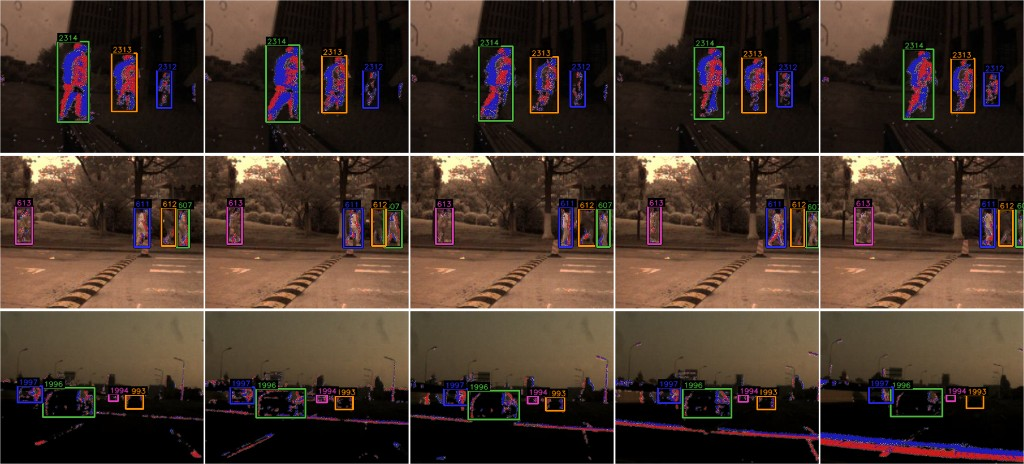
\includegraphics[width=\columnwidth]{tracking_result.png}
  \caption{Identity over three consecutive FEMOT frames. Salient event pixels are composited on the RGB frame. Each row keeps the same box identities: pedestrians walking at night, pedestrians crossing a road, and vehicles driving at night.}
  \label{fig:trackvis}
\end{figure}


\subsection{Limitation Analysis}
\label{sec:limit}

In our current tracker, association is formulated as local geometric matching: after the hypergraph-conditioned Mamba predicts the subsequent bounding box, matching with detections relies solely on IoU without accessing persistent identity records. Although appearance, group context and historical motion inform box prediction, these cues are not preserved as retrievable memory for subsequent matching. This mechanism suffers from ambiguous IoU overlaps caused by occlusion, crowded targets and target re-entry, which may lead to assignment conflicts and failed identity recovery for disappeared tracks. Equipping the tracker with temporal memory, such as persistent track queries or archived appearance and motion history, can enhance association while keeping the box prediction module intact.


\section{Conclusion}

This paper proposes two modules for frame-event multi-object tracking. A shared-MLP bidirectional HyLA block lets the RGB and event streams read each other inside the detector. The main module is a frame-level hypergraph: tracks that are close in space or similar in appearance are placed on one hyperedge, and the resulting group prior modulates the discretization step size $\Delta$ and the output matrix $C$ of a bidirectional Mamba, so that a target with difficult motion is predicted with guidance from its group. On both FEMOT and DSEC-MOT, the tracker improves over the MambaTrack baseline.

\FloatBarrier
\section*{LLM Usage Statement}

Grok 4.7 was used to polish the writing, check the grammar, and survey related work. 

{
    \small
    \bibliographystyle{ieeenat_fullname}
    \bibliography{main}
}

% Supplementary material is paper/supplementary.tex.
% Compile it separately. Do not \input it into this file.

\end{document}
